\documentclass{ximera}

\author{Anna Davis} \title{MTH 240 Homework 9} 

\begin{document}

\begin{abstract}

\end{abstract}
\maketitle
 \textit{Certificate due: 4/14/2021 at 11:59 p.m.}
 
\begin{problem}\label{prob:240HW9prob1}
Evaluate the indefinite integral.
  \begin{enumerate}
\item
$\int 5x^2+\sqrt{x}\,dx=\answer{\frac{5}{3}x^3+\frac{2}{3}x^{1.5}}+C$

\item
$\int e^x+\cos x\, dx=\answer{e^x+\sin x}+C$

\item
$\int \frac{x+x^2}{x}\,dx=\answer{x+0.5x^2}+C$
  \end{enumerate}
\end{problem}

\begin{problem}\label{prob:240HW9prob2}
Evaluate the definite integral.  Enter exact values; no decimal approximations.
  \begin{enumerate}
\item
$\int_1^5 4x+1\, dx=\answer{52}$

\item
$\int_{-\pi}^{\pi} \sin x\, dx=\answer{0}$

\item
$\int_{-1}^1 x^2\, dx=\answer{\frac{2}{3}}$

  \end{enumerate}
\end{problem}

\begin{problem}\label{prob:240HW9prob3}
Let $f(x)=-x^2-x+6$.  Use $L_4$ and follow the indicated steps to estimate the area under the curve on the interval $[-1,1]$.  
\begin{image}
   
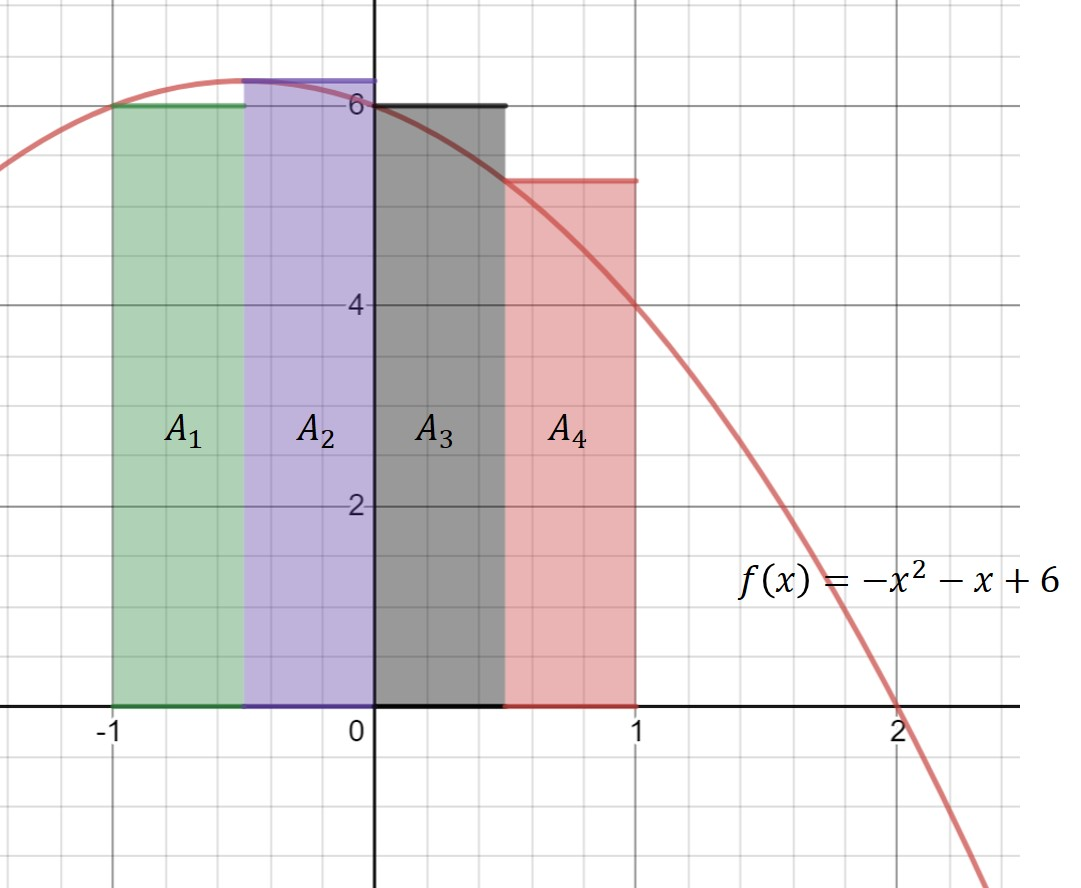
\includegraphics[height=1in]{MTH240HW9pic1.jpg}

\end{image}
Find the exact area of each rectangle.
$$A_1=\answer{3},\quad A_2=\answer{3.125},\quad A_3=\answer{3},\quad A_4=\answer{2.625}$$

Estimate the total area under the curve.
$$\mbox{Total Area Under the Curve }\approx \Sigma_{i=1}^{i=4}A_i=\answer{11.75}$$
\end{problem}


\end{document} 